% Fakesection Preamble-ish commands
\newcommand{\sectionbreak}{\clearpage}
\renewcommand*{\thefigure}{S\arabic{figure}}
\renewcommand*{\thetable}{S\arabic{table}}
\renewcommand*{\thepage}{S\arabic{page}}
\setcounter{page}{1}
\setcounter{figure}{0}
\setcounter{table}{0}
\onehalfspacing

% Fakesection Title page
\hspace{0pt}
\vfill
\begin{center}
    \huge
    Supporting Information

    \textit{for}

    Diversifying NOAH Supersequences with New HSQC-based Modules

    \vspace{1cm}

    \Large Jonathan R. J. Yong,\textsuperscript{1} {\=E}riks Kup{\v{c}}e,\textsuperscript{2} Tim D. W. Claridge\textsuperscript{1,}*

    \vspace{1cm}

    \large \textsuperscript{1} \textit{Chemistry Research Laboratory, Department of Chemistry, University of Oxford, Mansfield Road, Oxford, OX1 3TA, U.K.}

    \textsuperscript{2} \textit{Bruker UK Ltd., Banner Lane, Coventry, CV4 9GH, U.K.}

    * \texttt{tim.claridge@chem.ox.ac.uk}
\end{center}
\thispagestyle{empty}
\vfill
\hspace{0pt}
\newpage

% Fakesection Table of contents
\tableofcontents

\newpage

\section{Product operator analysis for NOAH modules}

\begin{figure}
    \centering
    % Inkscape
    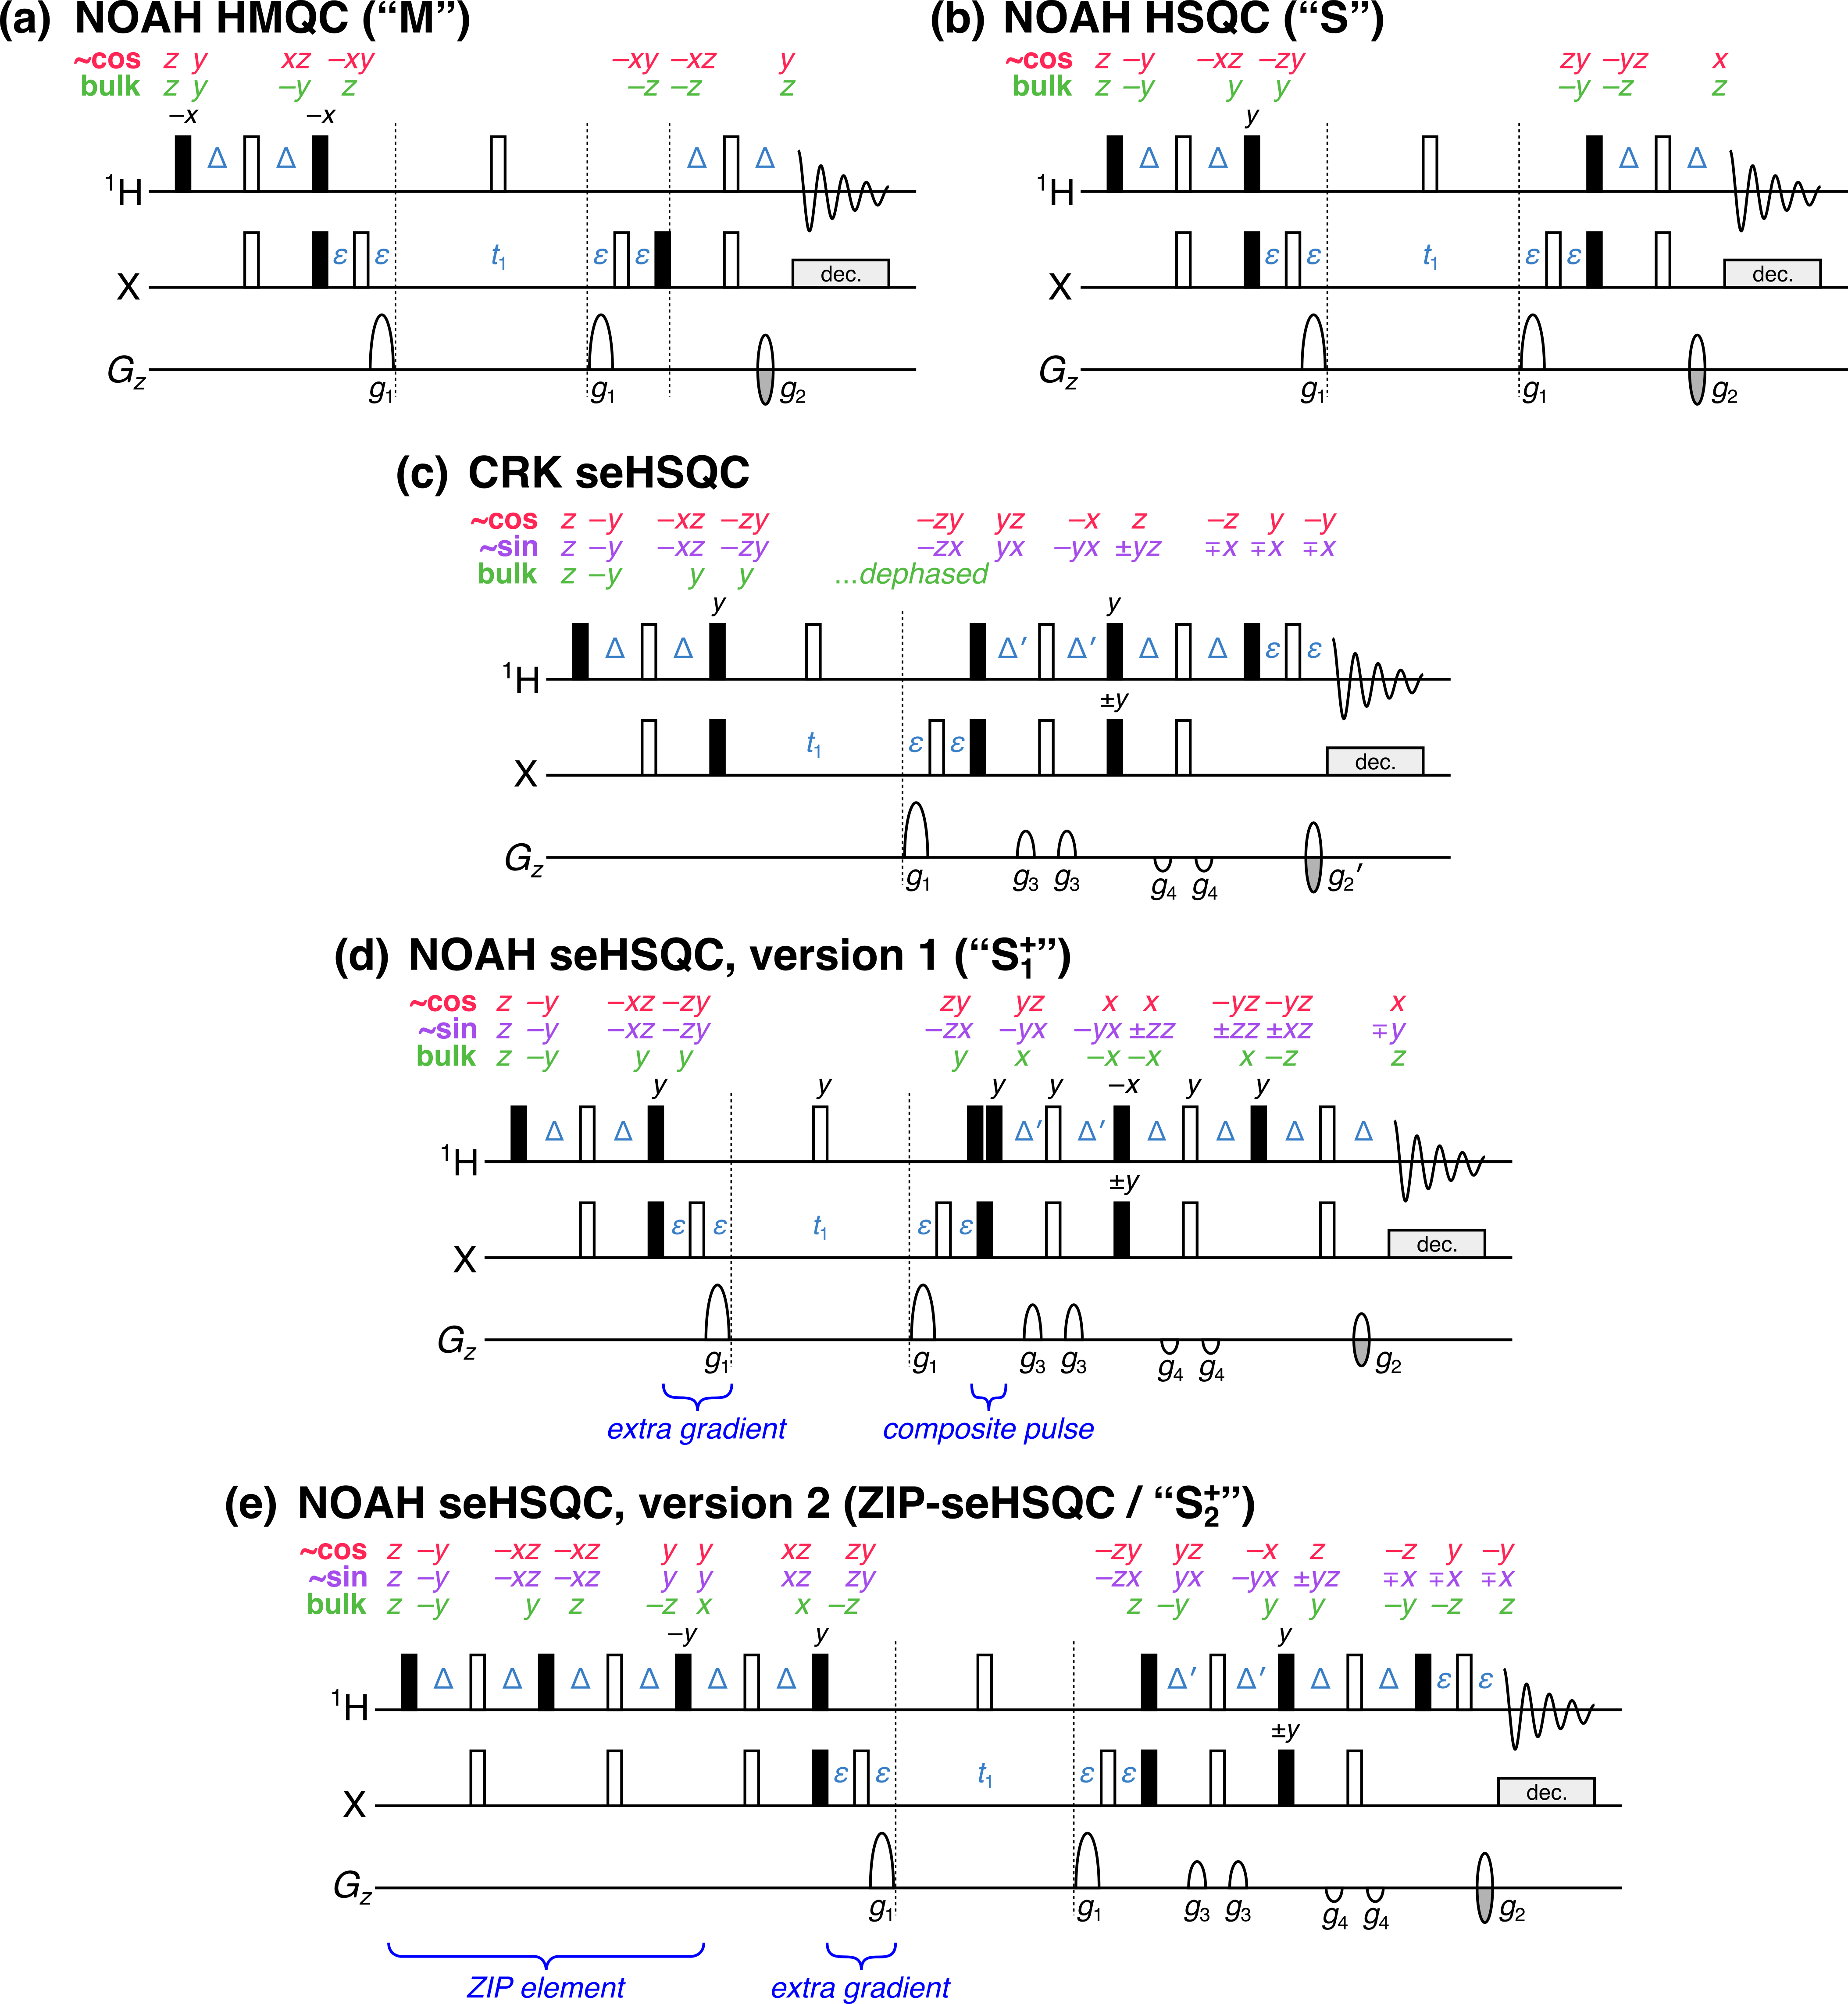
\includegraphics[width=0.8\textwidth]{./figures/pprogs_prodop.png}
    \caption{
        Product operators present at each stage of NOAH modules for an IS spin system.
        One-letter terms $m$ ($m \in \{x, y, z\}$) are shorthand for single-spin terms on proton, i.e.\ $\hat{I}_m$.
        Two-letter terms $mn$ are shorthand for two-spin terms on both the proton and heteronucleus, i.e.\ $2\hat{I}_m\hat{S}_n$.
        ``$\sim$cos'' represents the pathway for directly coupled proton magnetisation that is cosine-modulated after $t_1$: for the HMQC and HSQC, this is the only component that is detected.
        For the seHSQC, the sine-modulated component (labelled with ``$\sim$sin'') is also detected.
        ``bulk'' refers to the bulk magnetisation, i.e.\ protons that are not directly coupled to the heteronucleus.
        \textbf{(a)} NOAH HMQC.
        \textbf{(b)} NOAH HSQC.
        \textbf{(c)} NOAH seHSQC with ISR.
        Immediately following the ISR pulse sequence element, directly bonded protons are rotated onto $+y$, whereas the bulk magnetisation is rotated onto $+x$.
        Note that this analysis assumes $\Delta' = 1/(4\cdot\onejxh)$.
    }
    \label{fig:pprogs_prodop}
\end{figure}

\section{Multiplicity editing in seHSQC}

\begin{figure}
    \centering
    % done in Inkscape
    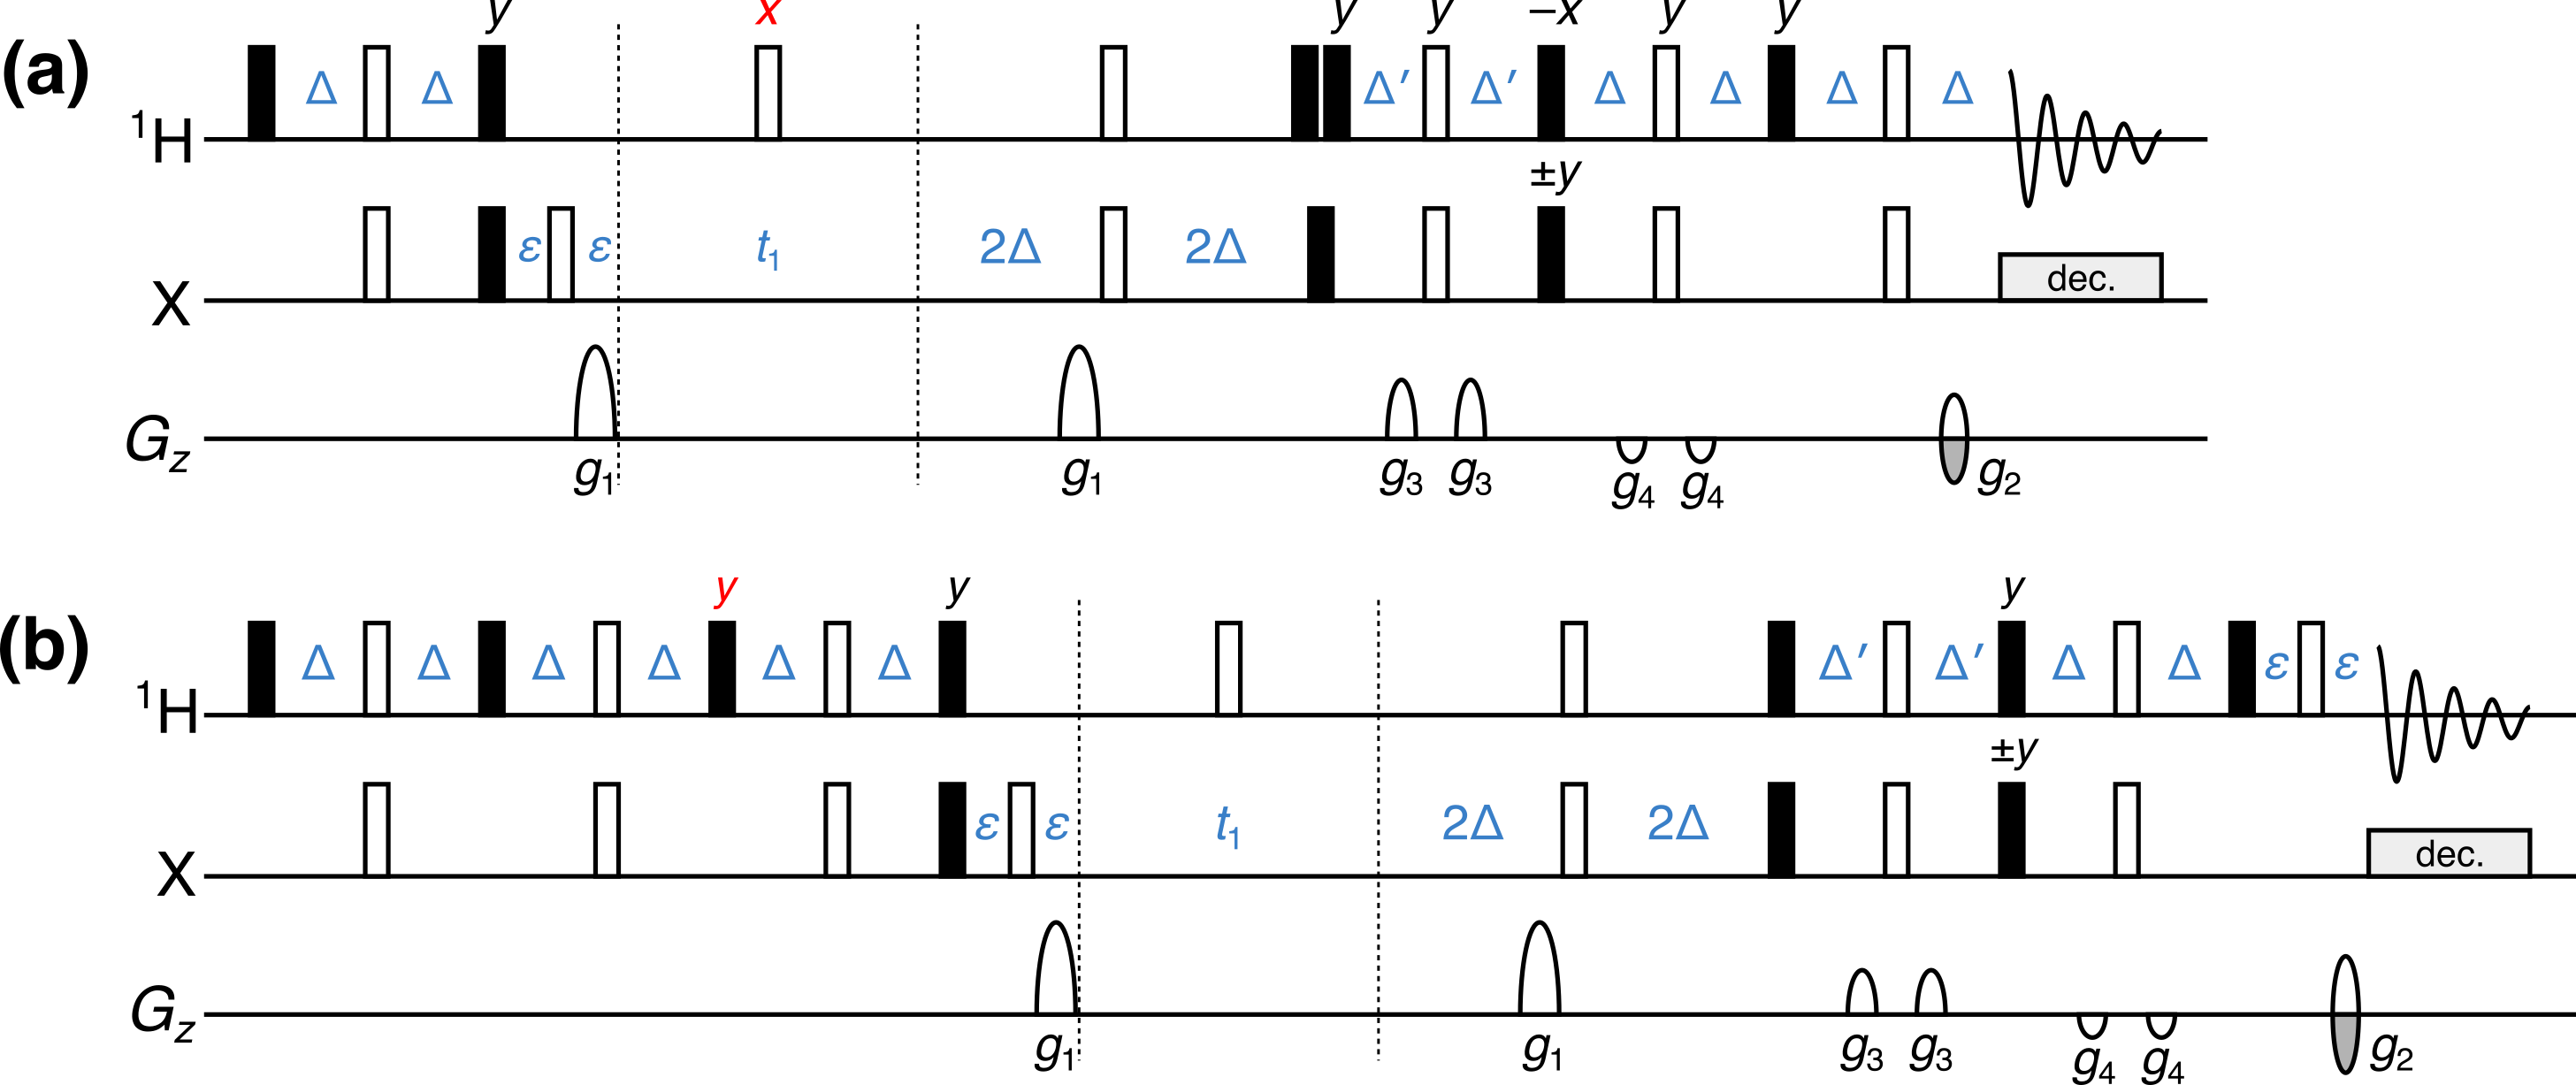
\includegraphics[width=0.8\textwidth]{./figures/mult_edit.png}
    \caption{
        Implementation of multiplicity editing in the new NOAH seHSQC module.
        \textbf{(a)} Unedited NOAH seHSQC, as presented in the main text.
        \textbf{(b)} Edited NOAH seHSQC (note the different phase in the third \proton{} \ang{90} pulse; this is needed to compensate for the extra \ang{180} in the editing period).
        Symbols have the same meaning as in \figref{pprogs} of the main text.
    }
    \label{fig:edited_sehsqc_pprog}
\end{figure}

\begin{figure}
    \centering
    % figures/edited_sn_comp.py
    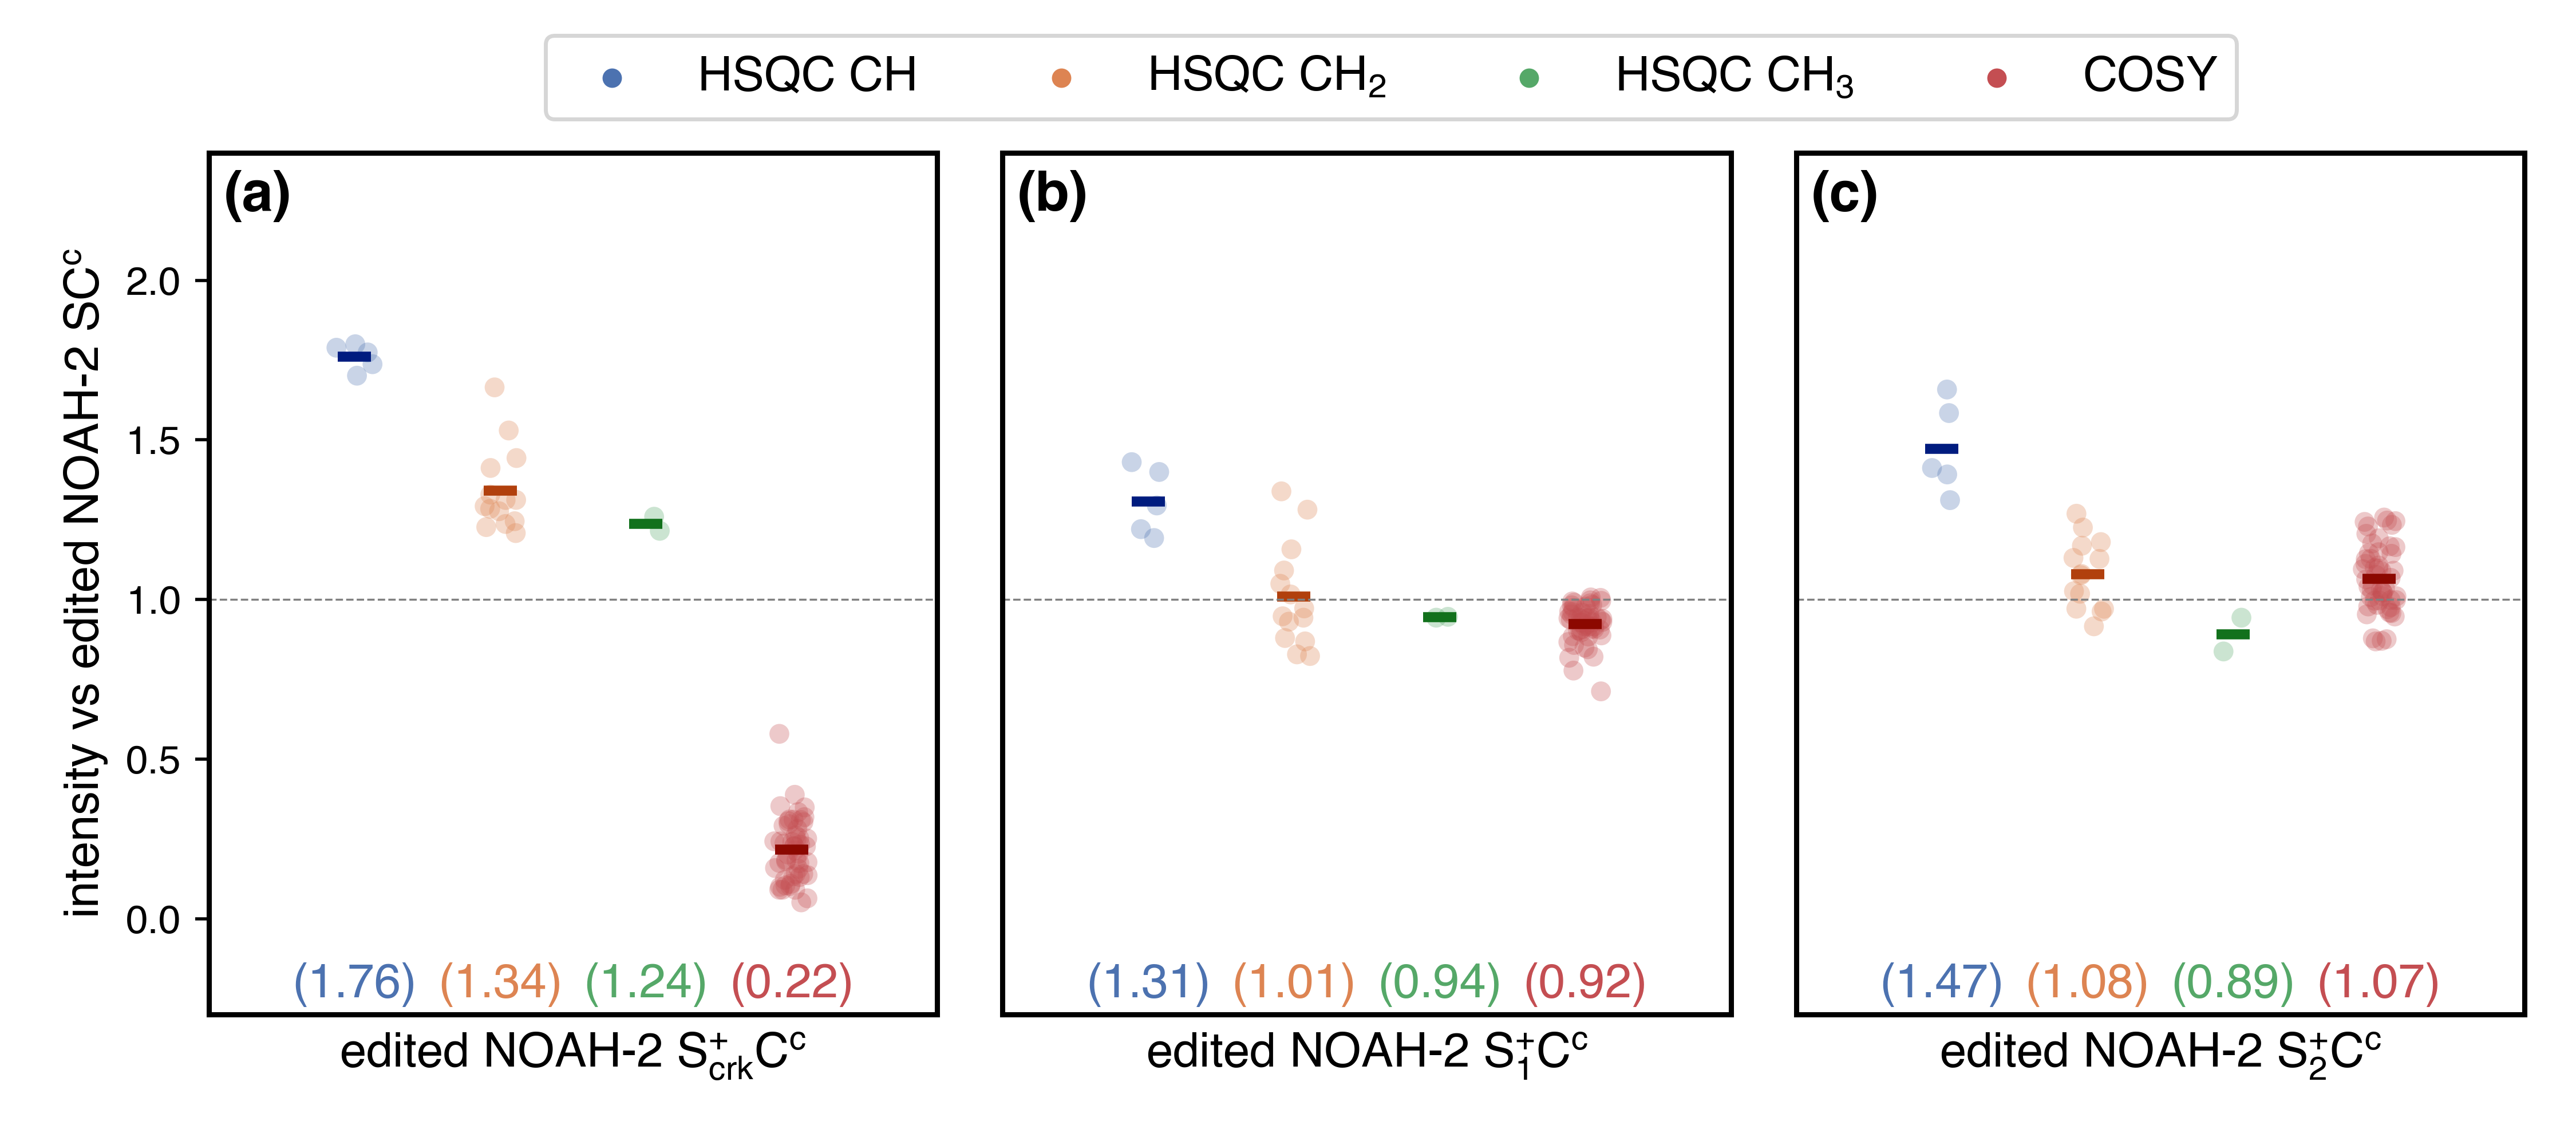
\includegraphics[width=0.8\textwidth]{./figures/edited_sn_comp.png}
    \caption{
        Sensitivity of edited seHSQC versus the NOAH HSQC/CLIP-COSY supersequence.
        \textbf{(a)} CRK edited seHSQC + CLIP-COSY.
        Although larger gains are observed in the HSQC, the COSY intensities are severely decreased.
        \textbf{(b)} NOAH edited seHSQC + CLIP-COSY.
        On average, sensitivity gains are observed in both the HSQC and COSY modules (except for HSQC \ce{CH3} peaks).
        \andro{}
    }
    \label{fig:edited_sn_comp}
\end{figure}

\section{Effect of setting \texorpdfstring{$\Delta' = 1/(4\cdot\onejch)$}{Delta' = 1/(4*1JCH)} in seHSQC}

The $\Delta'$ delay in the CRK and NOAH seHSQC sequences can be set to $1/(4\cdot\onejch)$ in order to optimise the sensitivity enhancement for \ce{CH} groups only.
The effects of doing so are shown here for the unedited and edited seHSQCs respectively.

\begin{figure}
    \centering
    % figures/combined_1_4j.py
    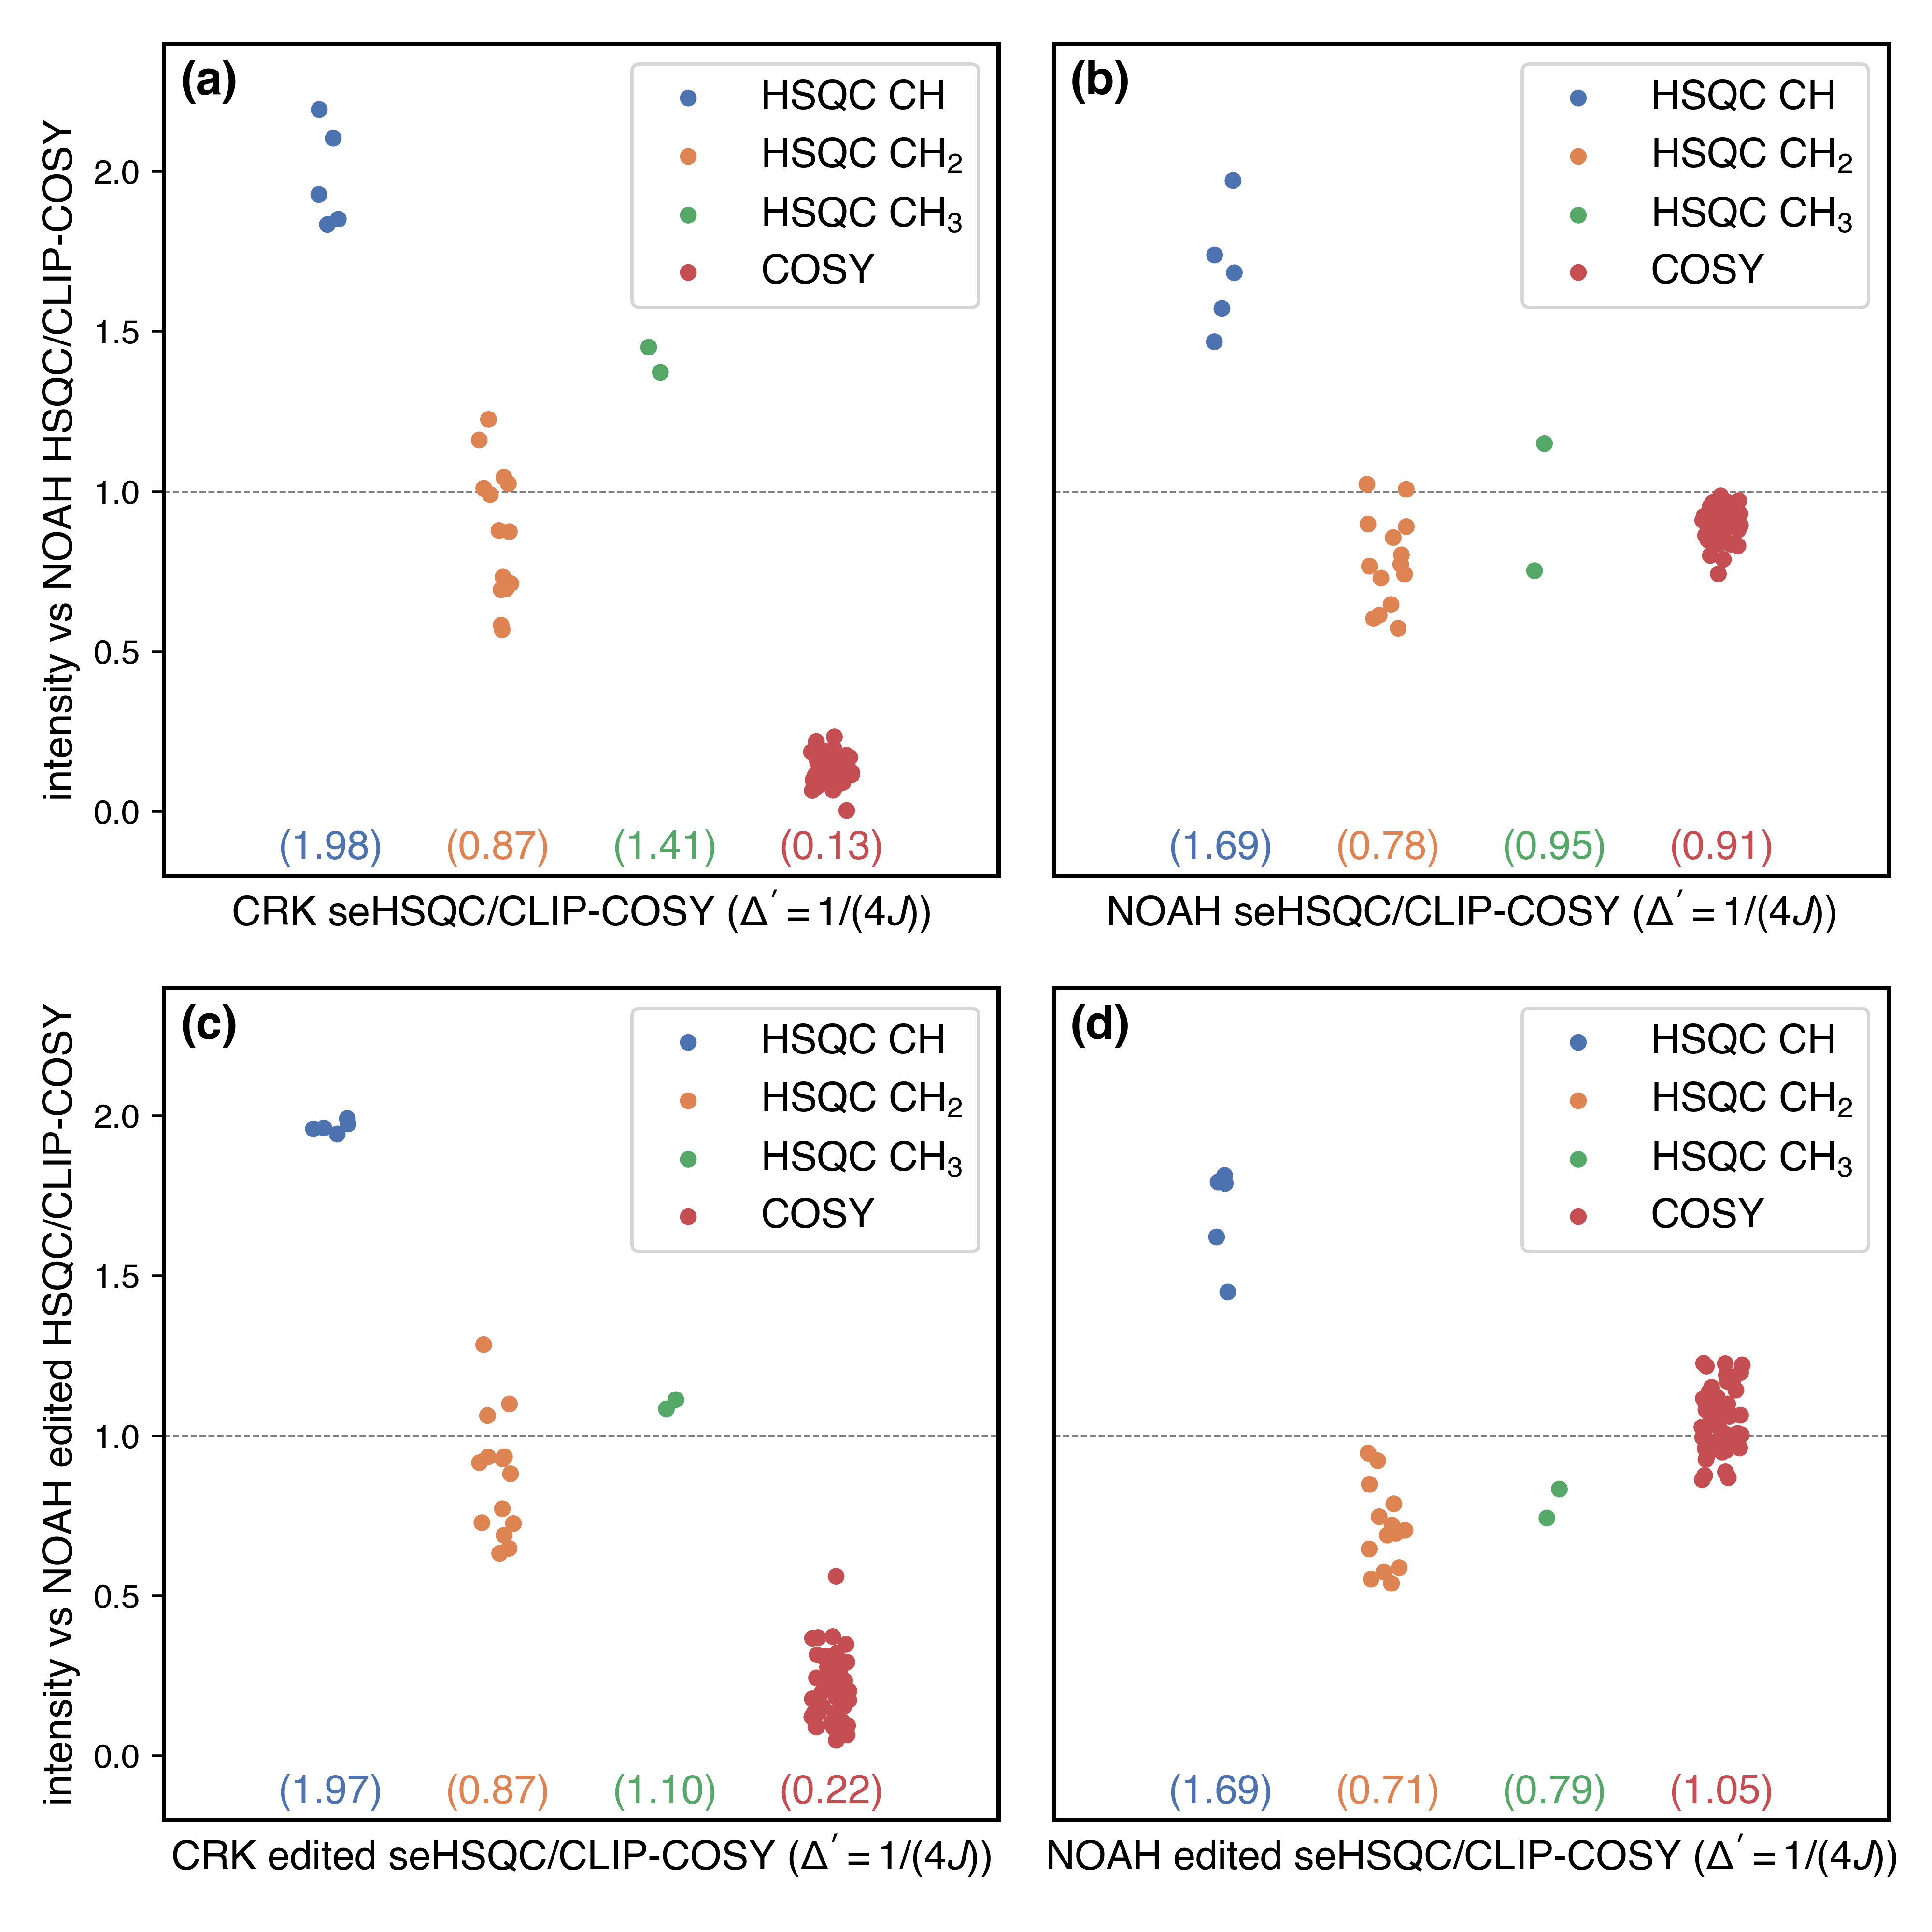
\includegraphics[width=0.8\textwidth]{./figures/combined_1_4j.png}
    \caption{
        Sensitivity of seHSQC sequences with $\Delta'$ set to $1/(4\cdot\onejch)$, versus the corresponding NOAH HSQC/CLIP-COSY supersequence (i.e.\ unedited for (a) and (b), edited for (c) and (d)).
        \textbf{(a)} CRK seHSQC + CLIP-COSY, without multiplicity editing.
        \textbf{(b)} NOAH seHSQC + CLIP-COSY, without multiplicity editing.
        \textbf{(c)} CRK seHSQC + CLIP-COSY, with multiplicity editing.
        \textbf{(d)} NOAH seHSQC + CLIP-COSY, with multiplicity editing.
        \andro{}
    }
    \label{fig:combined_1_4j}
\end{figure}

In particular, for the NOAH seHSQC, we note that the improvements in HSQC \ce{CH} sensitivity gained by moving from $\Delta' = 1/(8\cdot\onejch)$ to $\Delta' = 1/(4\cdot\onejch)$ are marginal (ca.\ 10\%).
At the same time, sensitivity \textit{losses} are observed for \ce{CH2} and \ce{CH3} peaks, likely due to pulse imperfections.

\section{Comparison of BIG-BIRD and ISR elements}

The BIG-BIRD element used here was ${45^\circ}_{45^\circ}(\proton{}) - 2\Delta - 180^\circ(\proton{},\carbon{}) - 2\Delta - {45^\circ}_{225^\circ}(\proton{})$ for the unedited NOAH seHSQC, where $\beta_\phi$ indicates a hard pulse with flip angle $\beta$ and phase $\phi$, and $\Delta = 1/(4\cdot\onejch)$.
For the edited NOAH seHSQC, the BIG-BIRD pulse phases are slightly modified to give ${45^\circ}_{315^\circ}(\proton{}) - 2\Delta - 180^\circ(\proton{},\carbon{}) - 2\Delta - {45^\circ}_{135^\circ}(\proton{})$.
These, and the ISR, have the same net effect on coupled and uncoupled proton magnetisation, as shown in \figref{pprogs_prodop}.
However, the ISR provides greater sensitivity in both the HSQC and downstream COSY.

\begin{figure}
    \centering
    % figures/bigbird.py
    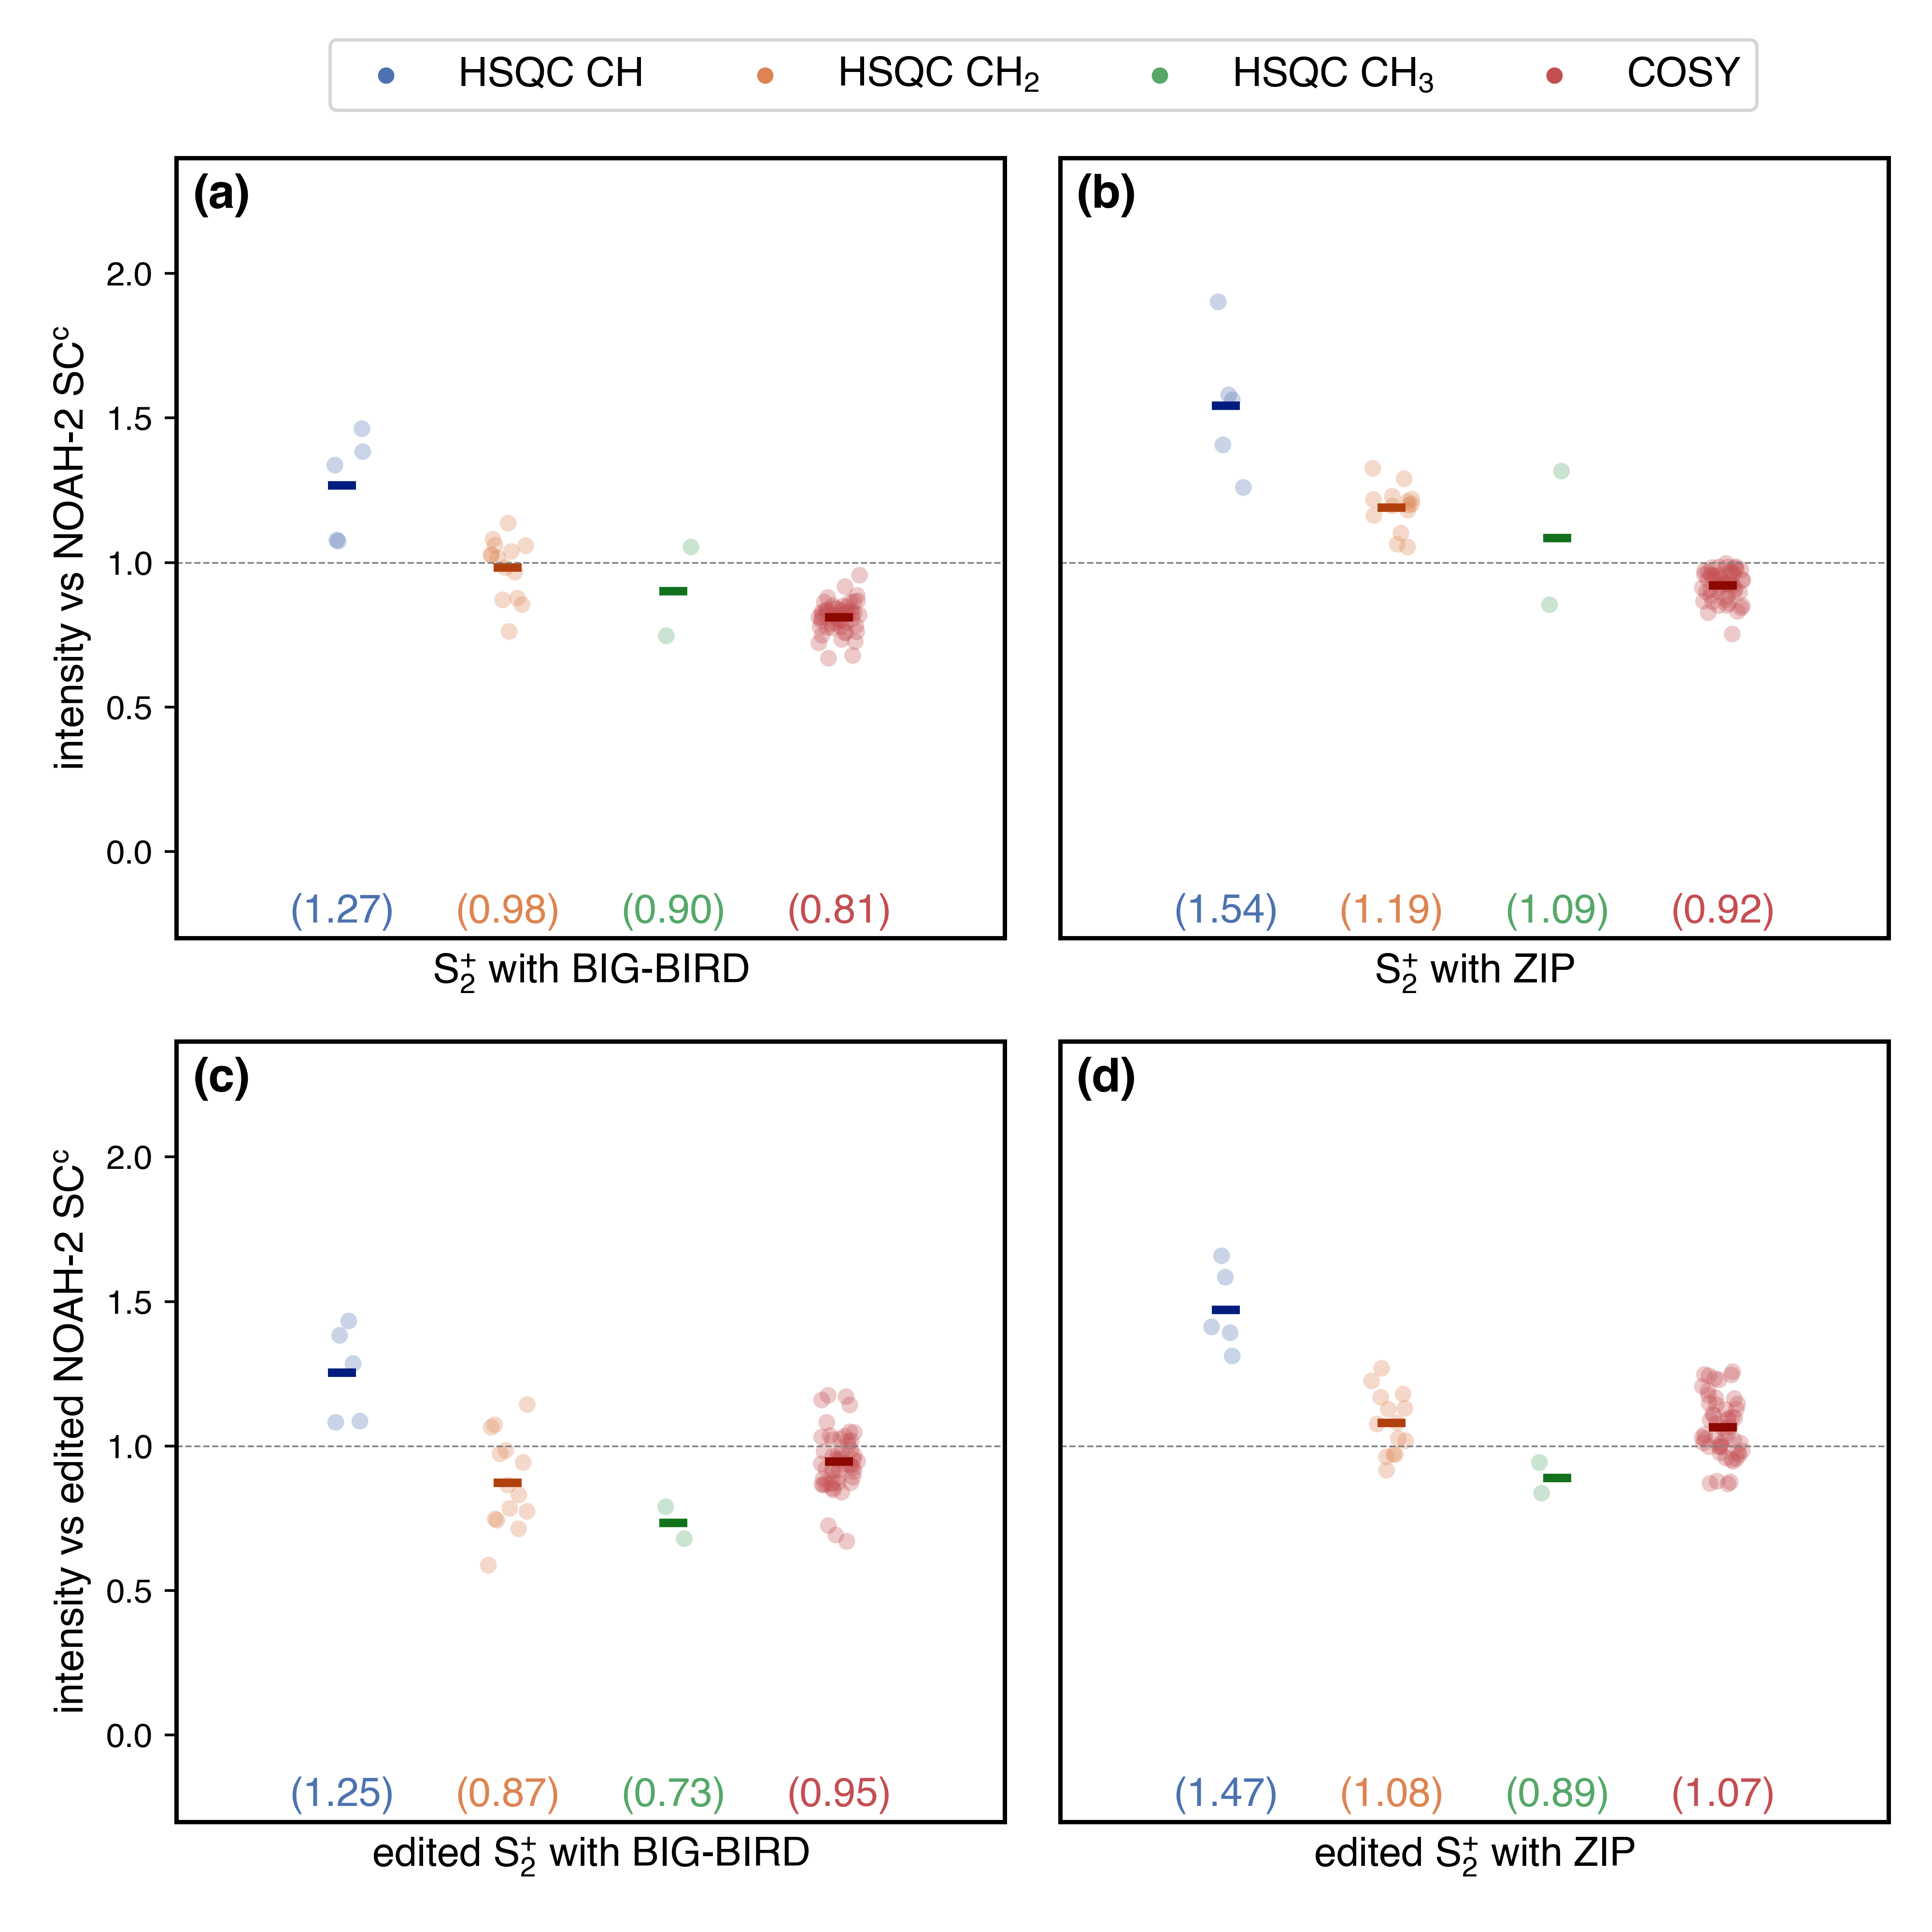
\includegraphics[width=0.8\textwidth]{./figures/bigbird.png}
    \caption{
        Sensitivity of NOAH seHSQC sequences with prepended BIG-BIRD and ISR elements, versus the corresponding NOAH HSQC/CLIP-COSY supersequence (i.e.\ unedited for (a) and (b), edited for (c) and (d)).
        \textbf{(a)} NOAH seHSQC with BIG-BIRD + CLIP-COSY, without multiplicity editing.
        \textbf{(b)} NOAH seHSQC with ISR + CLIP-COSY, without multiplicity editing.
        \textbf{(c)} NOAH seHSQC with BIG-BIRD + CLIP-COSY, with multiplicity editing.
        \textbf{(d)} NOAH seHSQC with ISR + CLIP-COSY, with multiplicity editing.
        \andro{}
    }
    \label{fig:bigbird}
\end{figure}


\section{Suppression of wing artefacts}

The origin of the ``wing'' artefacts in the final homonuclear modules can be most clearly seen from the following series of experiments involving the NOAH-3 \nitrogen{} seHSQC/\carbon{} seHSQC/CLIP-COSY (SpSpCc) supersequence.
Since the $f_1$ spectral windows of the two seHSQC modules are different, they lead to distinct sets of wing artefacts if the extra gradient before $t_1$ is not present.
\figref{wing_artefacts} focuses on the artefacts associated with intense methyl group peaks, but similar artefacts are observed for all other peaks, albeit with lower absolute intensities.

\begin{figure}
    \centering
    % figures/wing_artefacts.py
    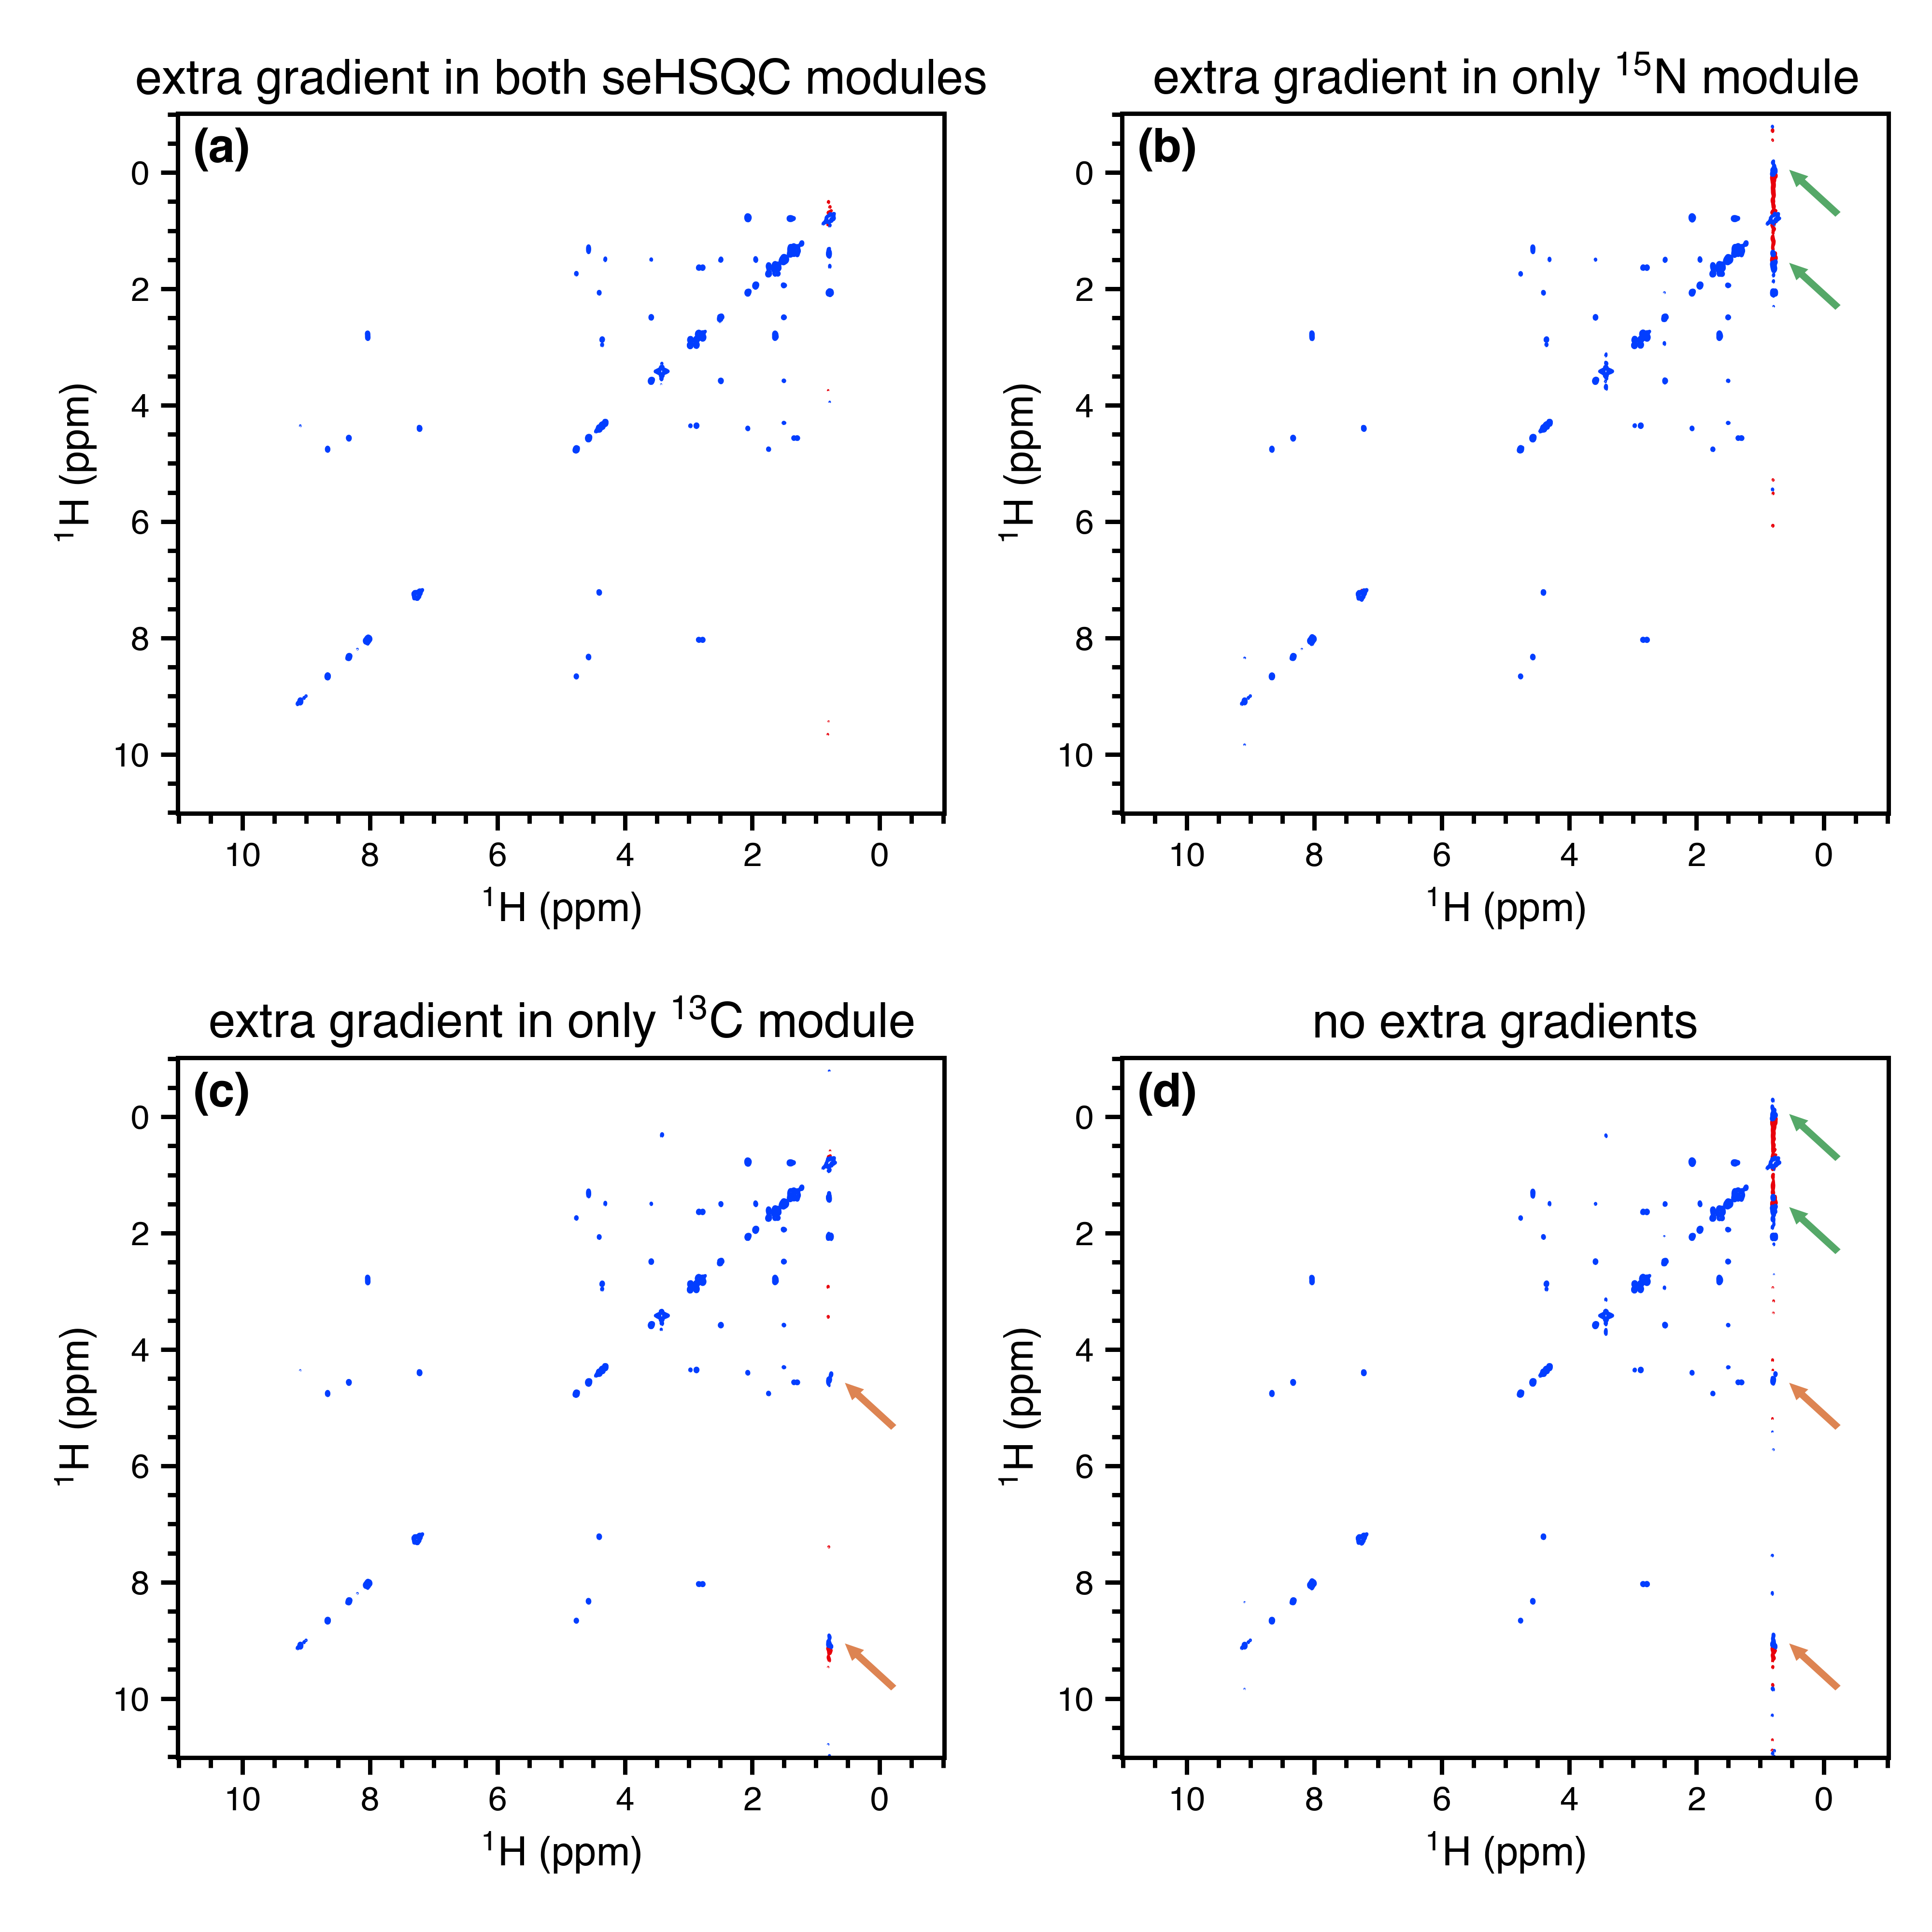
\includegraphics[width=0.8\textwidth]{./figures/wing_artefacts.png}
    \caption{
        CLIP-COSY spectra obtained from various forms of the NOAH-3 SpSpCc supersequence.
        Wing artefacts arising from the \nitrogen{} seHSQC are highlighted in orange; those arising from the \carbon{} seHSQC in green.
        Notice how (in this case) the former can easily be misinterpreted as a crosspeak, while the latter obscures genuine crosspeaks.
        \textbf{(a)} With the extra gradient inserted for both modules, i.e.\ no artefacts.
        \textbf{(b)} With an extra gradient in only the \nitrogen{} module, i.e.\ only the \carbon{} artefacts.
        \textbf{(c)} With an extra gradient in only the \carbon{} module.
        \textbf{(d)} With no extra gradients.
        \grami{}
    }
    \label{fig:wing_artefacts}
\end{figure}


\section{\texorpdfstring{\nitrogen{}}{15N} HSQC and line broadening}

For \nitrogen{}--\proton{} correlations, both the HMQC and the new seHSQC module are recommended as they keep the bulk magnetisation along $\pm z$ during the $t_1$ period.
The HSQC module places bulk magnetisation in the $xy$-plane, leading to $\jhh$ evolution; consequently, the amount of bulk magnetisation ``passed on'' to the downstream modules decreases as the \nitrogen{} $t_1$ is increased.
Since $t_1$ for each NOAH module is incremented in sync, this is manifested in downstream modules as a $t_1$-dependent decrease in amplitude, or $f_1$ line broadening after Fourier transformation, as shown in \figref{n15_linebroadening}.

\begin{figure}
    \centering
    % figures/n15_linebroadening.py
    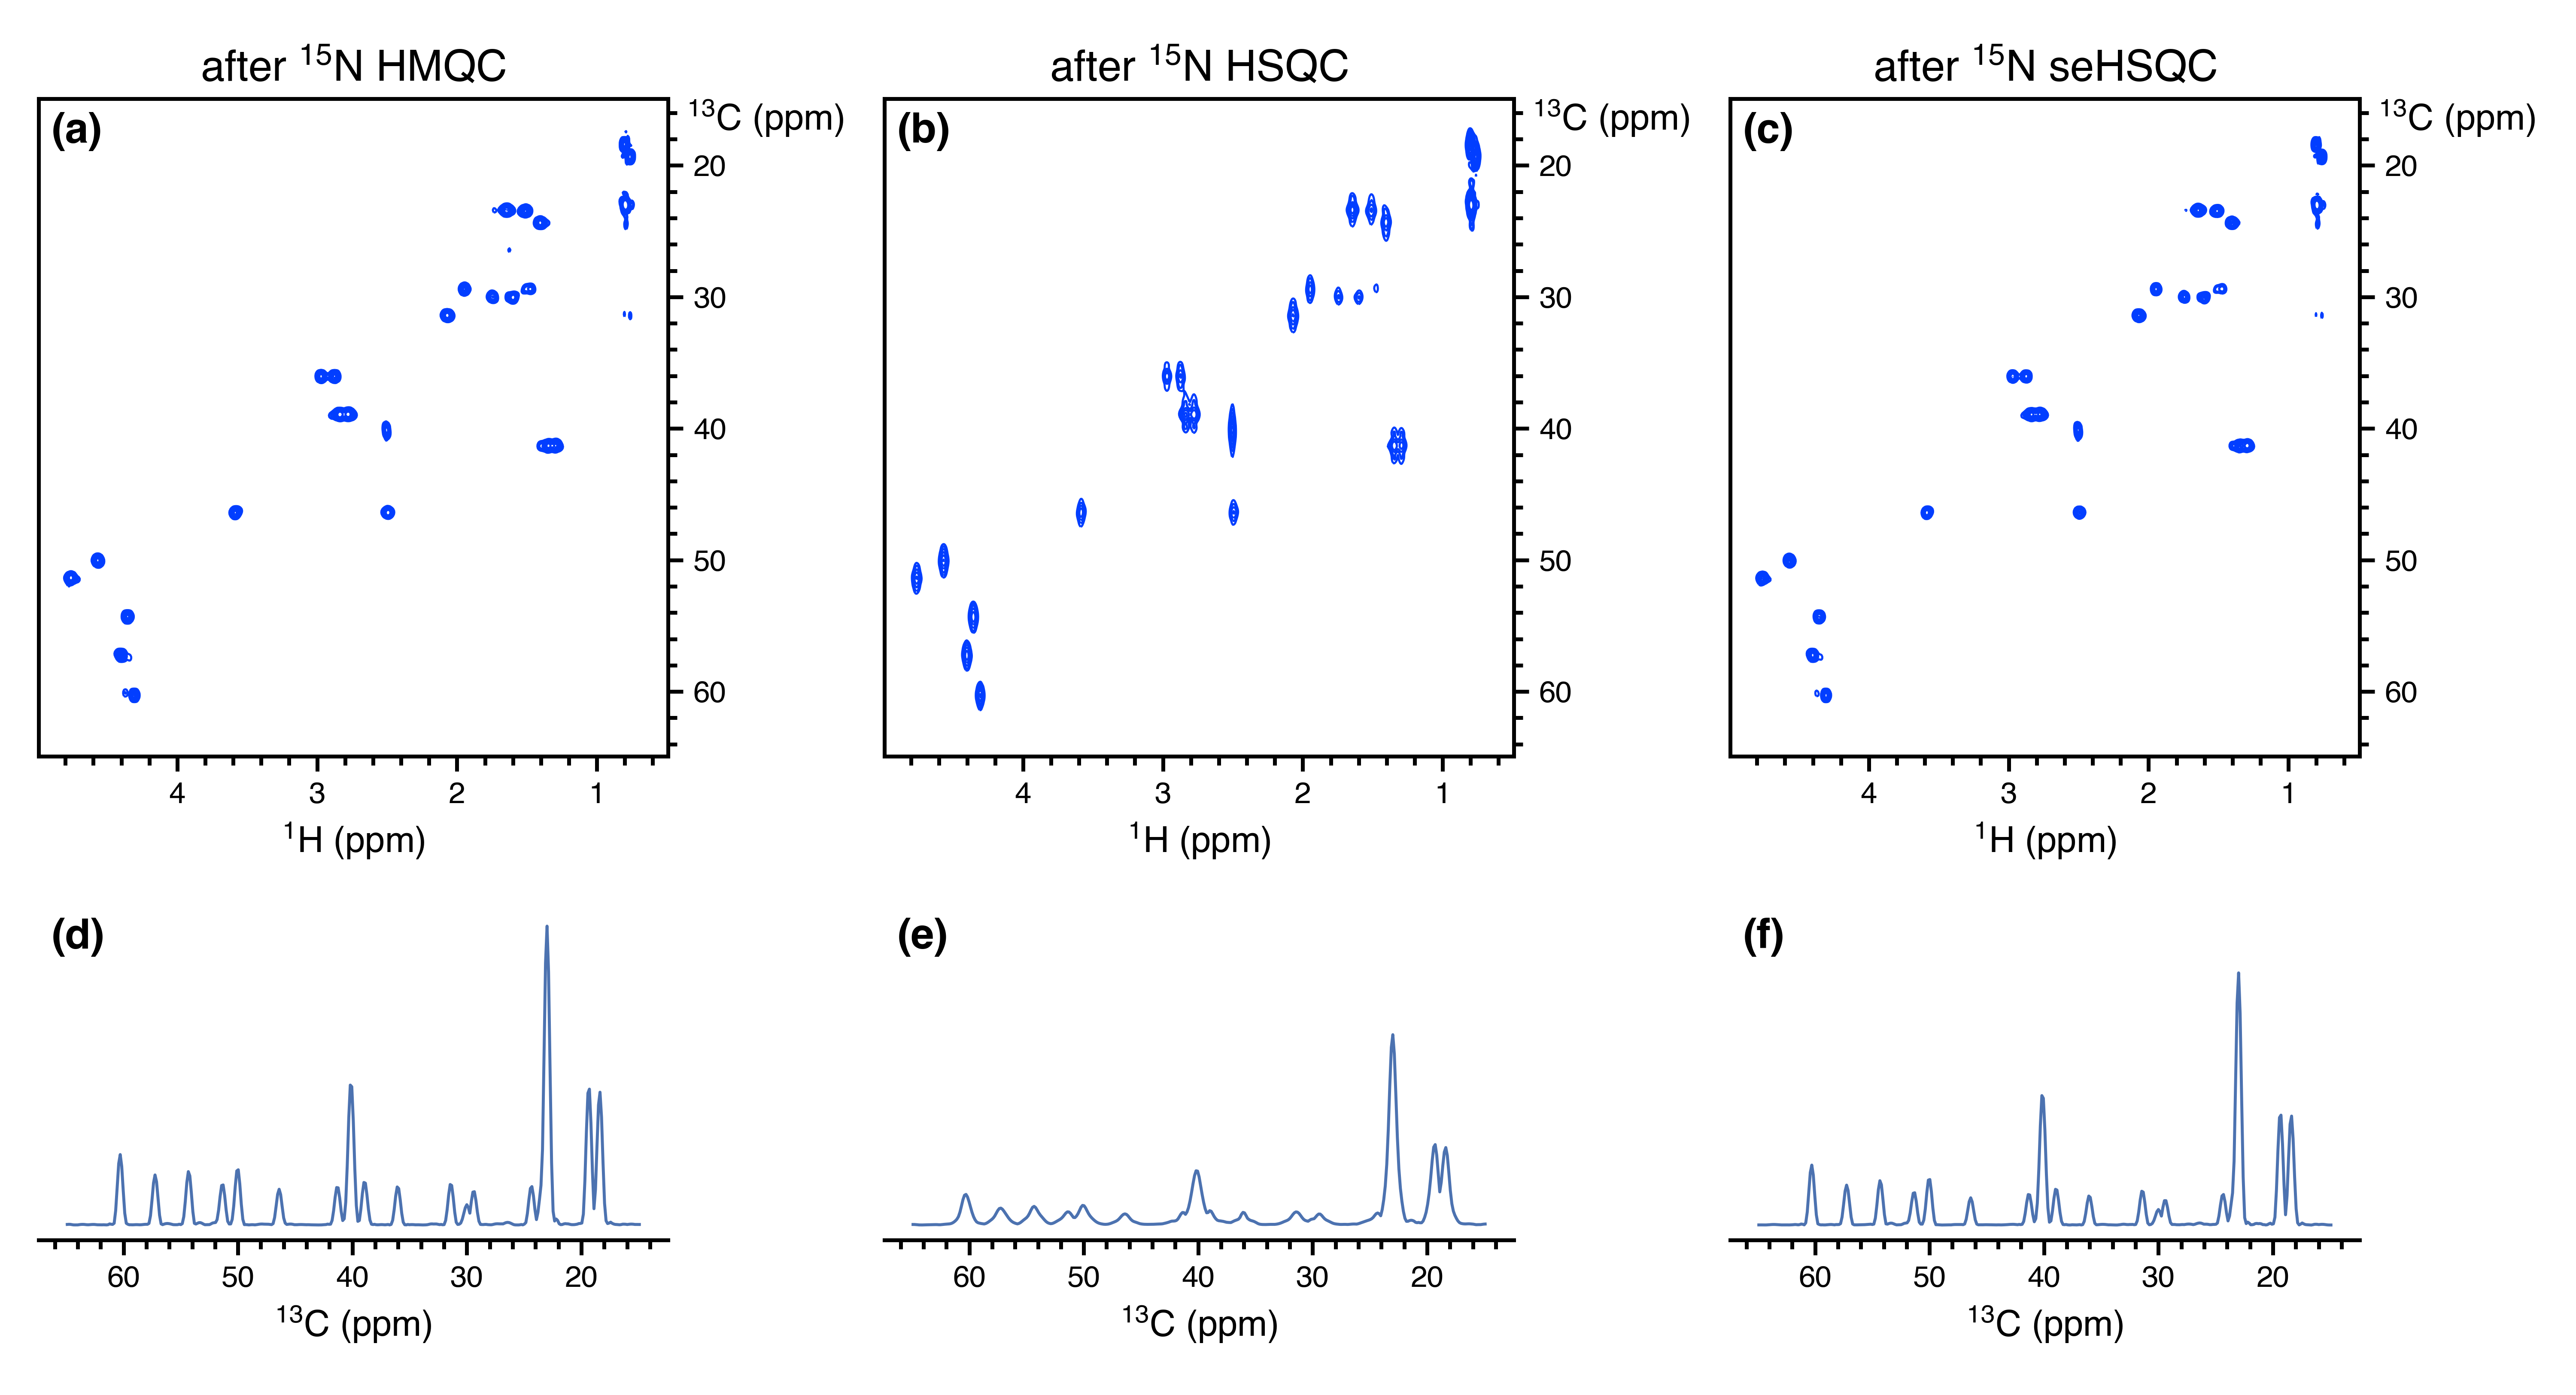
\includegraphics[width=\textwidth]{./figures/n15_linebroadening.png}
    \caption{
        \carbon{} seHSQC spectra obtained from NOAH-3 XSpCc (\nitrogen{} module + \carbon{} seHSQC + CLIP-COSY) supersequences.
        The \nitrogen{} spectral window was \SI{30}{ppm} and 256 $t_1$ increments were collected, corresponding to an indirect-dimension \nitrogen{} acquisition time of \SI{60.1}{\ms}.
        \textbf{(a)} X = HMQC.
        \textbf{(b)} X = HSQC.
        \textbf{(c)} X = seHSQC.
        \textbf{(d)}--\textbf{(f)} Projections of spectra \textbf{(a)}--\textbf{(c)} onto the $f_1$ axis.
        Note the $f_1$ line broadening in (b) and (e).
        \grami{}
    }
    \label{fig:n15_linebroadening}
\end{figure}

This line broadening also leads to a substantial sensitivity loss (almost 65\% in \figref{n15_linebroadening}).
The extent of the line broadening depends on the acquisition time, and is particularly pronounced for long acquisition times, i.e.\ small \nitrogen{} spectral windows.
In our experience, at \nitrogen{} acquisition times of ca.\ \SI{5}{\ms} the effect is almost indiscernible.
Such a short acquisition time would lead to poor resolution in the \nitrogen{} dimension itself, which may or may not be tolerable.
Of course, this issue can be entirely avoided by using either the HMQC or seHSQC.

\section{Effect of lengthened gradients in \texorpdfstring{\nitrogen{}}{15N} experiments}

\begin{figure}
    \centering
    % figures/cnst16_diff.py
    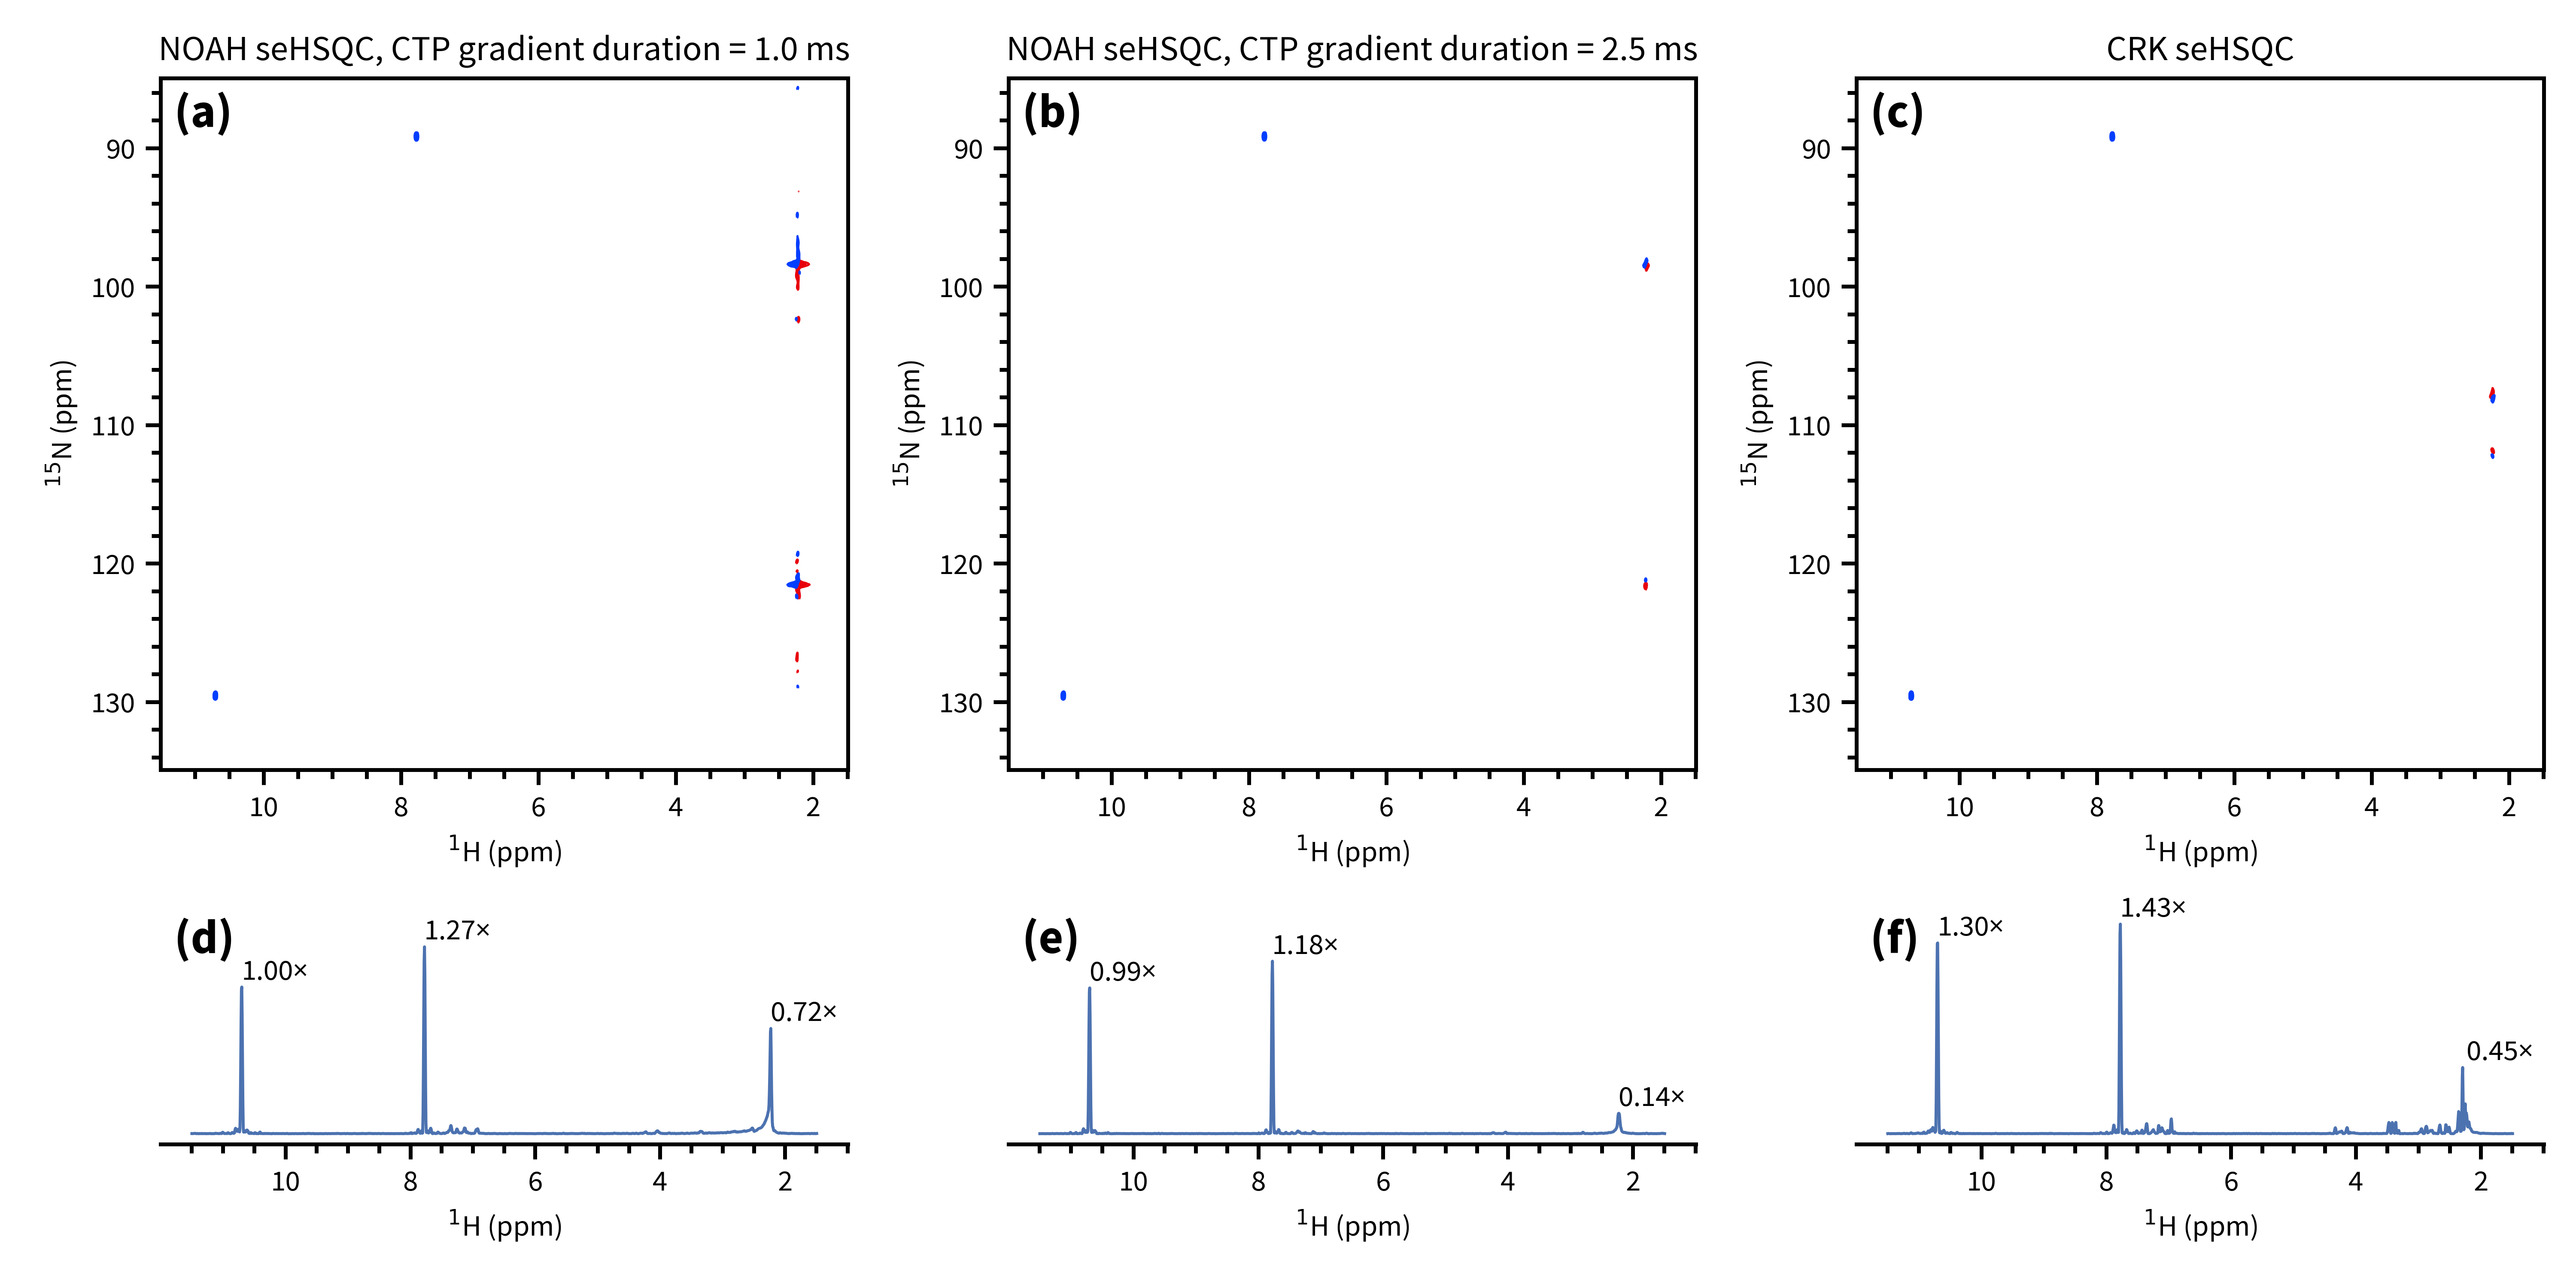
\includegraphics[width=\textwidth]{./figures/cnst16_diff.png}
    \caption{
        \nitrogen{} seHSQC spectra obtained using the NOAH and CRK methods.
        The peaks at 7.8 and \SI{10.7}{\ppm} (\proton{} shifts) are genuine crosspeaks; the mixed-phase peaks at \SI{2.2}{\ppm} are artefacts.
        \textbf{(a)} NOAH seHSQC, with original CTP gradients of \SI{1}{\ms}.
        \textbf{(b)} NOAH seHSQC, with longer CTP gradients of \SI{1}{\ms}.
        \textbf{(c)} Standalone CRK seHSQC with \SI{1}{\ms} CTP gradients.
        \textbf{(d)}--\textbf{(f)} Projections of spectra \textbf{(a)}--\textbf{(c)} onto the $f_2$ axis.
        The numbers indicate relative peak heights (normalised against the \SI{10.7}{\ppm} peak in (d)).
        \zolmi{}
    }
    \label{fig:cnst16_diff}
\end{figure}

The lengthening of CTP gradients from \SI{1}{\ms} to \SI{2.5}{\ms} is aimed at cleaning up artefacts arising from bulk magnetisation that is not properly returned to $+z$ at the end of the sequence.
\figref{cnst16_diff} shows exactly how effective this strategy is.
In (d), where the CTP gradients have their original duration, the artefacts have comparable intensity to the desired peaks.
When the gradients are lengthened in (e), the crosspeak intensities are almost unaffected (with losses of $<10\%$ arising perhaps from relaxation and diffusion).
However, the artefacts are suppressed by a factor of 5 or more.
Although this suppression is not complete, this should not be interpreted as a weakness of the new NOAH seHSQC module, as these artefacts are also visible in the CRK seHSQC (f).
Indeed, every \nitrogen{}--\proton{} experiment we tested has at least \textit{some} artefact intensity in this region.

\section{Effect of \texorpdfstring{$k$}{k}-scaling}

... both signal and artefact intensity, plus example spectra

\section{HSQC-TOCSY SNR comparisons}

... including Parella work

\section{Other example spectra}

...

\section{Pulse programmes}

...

\section{Processing scripts}

...
